% =============================================================================
% Chapter 8: Simulation and Experimental Results
% Pit-Viper-Inspired Infrared-Thermal and Visual Sensor Fusion
% for Nocturnal UAV Navigation
% =============================================================================
\selectlanguage{hebrew}

\section{תוצאות סימולציה וניסויים}
\label{sec:ch08_results}

\subsection{הגדרת סביבת הסימולציה ומערך הניסוי}
\label{sec:ch08_experimental_setup}

בפרק זה אנו מציגים תוצאות ניסוייות מקיפות של מערכת \en{TVF} שפותחה במסגרת מחקר זה. הניסויים בוצעו בשתי סביבות משלימות: סביבת סימולציה מבוקרת המאפשרת חזרתיות מלאה של תנאי הניסוי, וסביבת שטח אמיתית הכוללת תנאי לילה משתנים. סביבת הסימולציה מבוססת על פלטפורמת \en{Gazebo} עם תוסף \en{ignition} המדמה מצלמה תרמית ברזולוציית 640x512 פיקסלים וטווח ספקטרלי של 7.5-13.5 מיקרומטר. מודל הסימולציה התרמית כולל פליטת חום מגופים חמים, החזרי חום ממשטחים, והנחתת אות באטמוספירה.

מערך הניסוי בשטח כלל 12 משימות טיסה ליליות שבוצעו בשטח פתוח בנגב המערבי בתנאי תאורה טבעיים הנעים בין 0.05 ל-50 \en{lux}. כל משימה כללה מסלול טיסה באורך 500-800 מטרים בגובה 15-30 מטרים, תוך מעבר על פני מכשולים טבעיים (עצים, סלעים) ומלאכותיים (גדרות, עמודים). נתוני האמת (\en{ground truth}) נאספו באמצעות מערכת \en{RTK GPS} בדיוק של 2.5 ס"מ ויחידת \en{IMU} מדויקת בתדר 400 הרץ.

המערכת הושוותה מול ארבע שיטות ייחוס מובילות: \en{ORB-SLAM3} במצב חזותי בלבד (\cite{MurArtal2015ORB}), \en{VINS-Mono} (\cite{Kalman1960}), \en{LOAM} (\cite{Zhang2014LOAM}), וגרסה מותאמת של \en{ORB-SLAM3} המשלבת מידע תרמי ברמת התכונות. כל השיטות הורצו על אותה פלטפורמת חומרה (\en{Jetson Orin NX}) עם אותם פרמטרי כיול, תוך שמירה על תנאי ניסוי זהים.

\subsection{מערך נתונים לילי: איסוף ואנוטציה}
\label{sec:ch08_dataset}

כחלק ממחקר זה נאסף מערך נתונים ייעודי לניווט רחפנים לילי הכולל זוגות תמונות חזותיות-תרמיות מתואמות. מערך הנתונים כולל 12,500 זוגות תמונות מ-12 משימות טיסה שונות, המכסות מגוון רחב של תנאי תאורה (0.05-50 \en{lux}), סוגי שטח (מדבר, עירוני, חקלאי), ועונות שנה. כל תמונה כוללת חותמת זמן מדויקת ופרמטרי כיול מלאים.

תהליך האנוטציה בוצע על ידי צוות של שלושה מומחים, שסימנו 8,423 מכשולים בסך הכל בקטגוריות הבאות: הולכי רגל (1,847), כלי רכב (1,234), עצים (2,891), עמודים (1,452), וגדרות (999). מהימנות בין-סוקרים (\en{inter-annotator reliability}) נמדדה באמצעות מדד \en{Cohen's Kappa} והגיעה ל-0.89, המעיד על עקביות גבוהה באנוטציה.

\subsection{מדדי הערכה}
\label{sec:ch08_metrics}

להערכת ביצועי המערכת השתמשנו במגוון מדדים כמותיים ואיכותניים. מדדי איכות המיזוג כוללים את \en{PSNR (Peak Signal-to-Noise Ratio)} ו-\en{SSIM (Structural Similarity Index)}:

\begin{equation}
\text{PSNR} = 10 \log_{10} \left( \frac{\max(I)^2}{\frac{1}{MN} \sum_{i,j} (I_{ij} - \hat{I}_{ij})^2} \right)
\label{eq:ch08_psnr}
\end{equation}

\begin{equation}
\text{SSIM}(x, y) = \frac{(2\mu_x \mu_y + C_1)(2\sigma_{xy} + C_2)}{(\mu_x^2 + \mu_y^2 + C_1)(\sigma_x^2 + \sigma_y^2 + C_2)}
\label{eq:ch08_ssim}
\end{equation}

כאשר $\mu_x, \mu_y$ הם ממוצעי העוצמות, $\sigma_x^2, \sigma_y^2$ הן השונויות, $\sigma_{xy}$ היא השונות המשותפת, ו-$C_1, C_2$ הם קבועי ייצוב. מדדי דיוק הניווט כוללים את \en{ATE (Absolute Trajectory Error)} ו-\en{RPE (Relative Pose Error)}:

\begin{equation}
\text{ATE} = \sqrt{\frac{1}{N} \sum_{i=1}^N \| \mathbf{T}_{\text{est}, i}^{-1} \cdot \mathbf{T}_{\text{gt}, i} \|_F^2}
\label{eq:ch08_ate}
\end{equation}

כאשר $\mathbf{T}_{\text{est}, i}$ ו-$\mathbf{T}_{\text{gt}, i}$ הם מסלולי האומדן והאמת בהתאמה, ו-$\|\cdot\|_F$ היא נורמת \en{Frobenius}. מדדי ביצועי זמן אמת כוללים את זמן ההשהיה הכולל, קצב העדכון, וצריכת ההספק.

\subsection{תוצאות מיזוג תמונות: ניתוח כמותי ואיכותני}
\label{sec:ch08_fusion_results}

תוצאות מיזוג התמונות הוערכו על מערך הנתונים הלילי שנאסף. טבלה \ref{tab:ch08_fusion_metrics} מציגה השוואה כמותית בין שיטות המיזוג השונות על פני ארבע רמות תאורה מייצגות.

\begin{table*}[htbp]
\centering
\caption{השוואת מדדי איכות מיזוג תמונות בשיטות שונות בתנאי תאורה משתנים.}
\label{tab:ch08_fusion_metrics}
\adjustbox{max width=\columnwidth}{%
\begin{tabular}{@{}lcccc@{}}
\toprule
\textbf{שיטה} & \textbf{0.1 lux} & \textbf{1 lux} & \textbf{10 lux} & \textbf{50 lux} \\
\midrule
\multicolumn{5}{c}{\textbf{PSNR [\en{dB}] $\uparrow$}} \\
\midrule
תמונה חזותית בלבד & 8.2 & 15.3 & 28.7 & 34.2 \\
תמונה תרמית בלבד & 22.1 & 22.5 & 22.8 & 23.0 \\
מיזוג ממוצע פשוט & 18.5 & 21.9 & 27.4 & 31.8 \\
מיזוג מבוסס \en{DWT} & 20.3 & 23.1 & 28.9 & 33.1 \\
מיזוג מבוסס רשת קשב צולב & 24.8 & 26.2 & 30.5 & 34.8 \\
\textbf{מיזוג אדפטיבי (\en{TVF})} & \textbf{26.1} & \textbf{27.8} & \textbf{31.2} & \textbf{35.3} \\
\midrule
\multicolumn{5}{c}{\textbf{SSIM $\uparrow$}} \\
\midrule
תמונה חזותית בלבד & 0.12 & 0.45 & 0.82 & 0.91 \\
תמונה תרמית בלבד & 0.68 & 0.69 & 0.70 & 0.70 \\
מיזוג ממוצע פשוט & 0.52 & 0.63 & 0.78 & 0.86 \\
מיזוג מבוסס \en{DWT} & 0.61 & 0.71 & 0.83 & 0.89 \\
מיזוג מבוסס רשת קשב צולב & 0.74 & 0.78 & 0.86 & 0.92 \\
\textbf{מיזוג אדפטיבי (\en{TVF})} & \textbf{0.79} & \textbf{0.82} & \textbf{0.88} & \textbf{0.93} \\
\bottomrule
\end{tabular}%
}
\end{table*}

התוצאות מראות ששיטת המיזוג האדפטיבי (\en{TVF}) משיגה ביצועים עדיפים בכל תנאי התאורה, עם שיפור משמעותי במיוחד בתנאי חושך קיצוני (0.1 \en{lux}). בתנאים אלה, שיטת \en{TVF} משיגה \en{PSNR} של 26.1 \en{dB} לעומת 8.2 \en{dB} לתמונה חזותית בלבד ו-22.1 \en{dB} לתמונה תרמית בלבד. השיפור נובע מהמשקל האדפטיבי $\alpha(t)$ המעניק עדיפות למידע התרמי בתנאי חושך, תוך שמירה על מידע חזותי בתנאי תאורה טובים.

איור \ref{fig:adaptive_fusion_example} מציג דוגמאות איכותניות למיזוג בתנאי תאורה שונים. ניתן לראות כי בתנאי חושך מוחלט (0.1 \en{lux}), התמונה החזותית כמעט שחורה לחלוטין, בעוד שהתמונה התרמית חושפת פרטים עשירים של הסביבה. המיזוג האדפטיבי משלב את המידע משני המקורות באופן אופטימלי, תוך שמירה על פרטים תרמיים חשובים והוספת מרקם חזותי היכן שזמין.

\begin{figure*}[htbp]
\centering
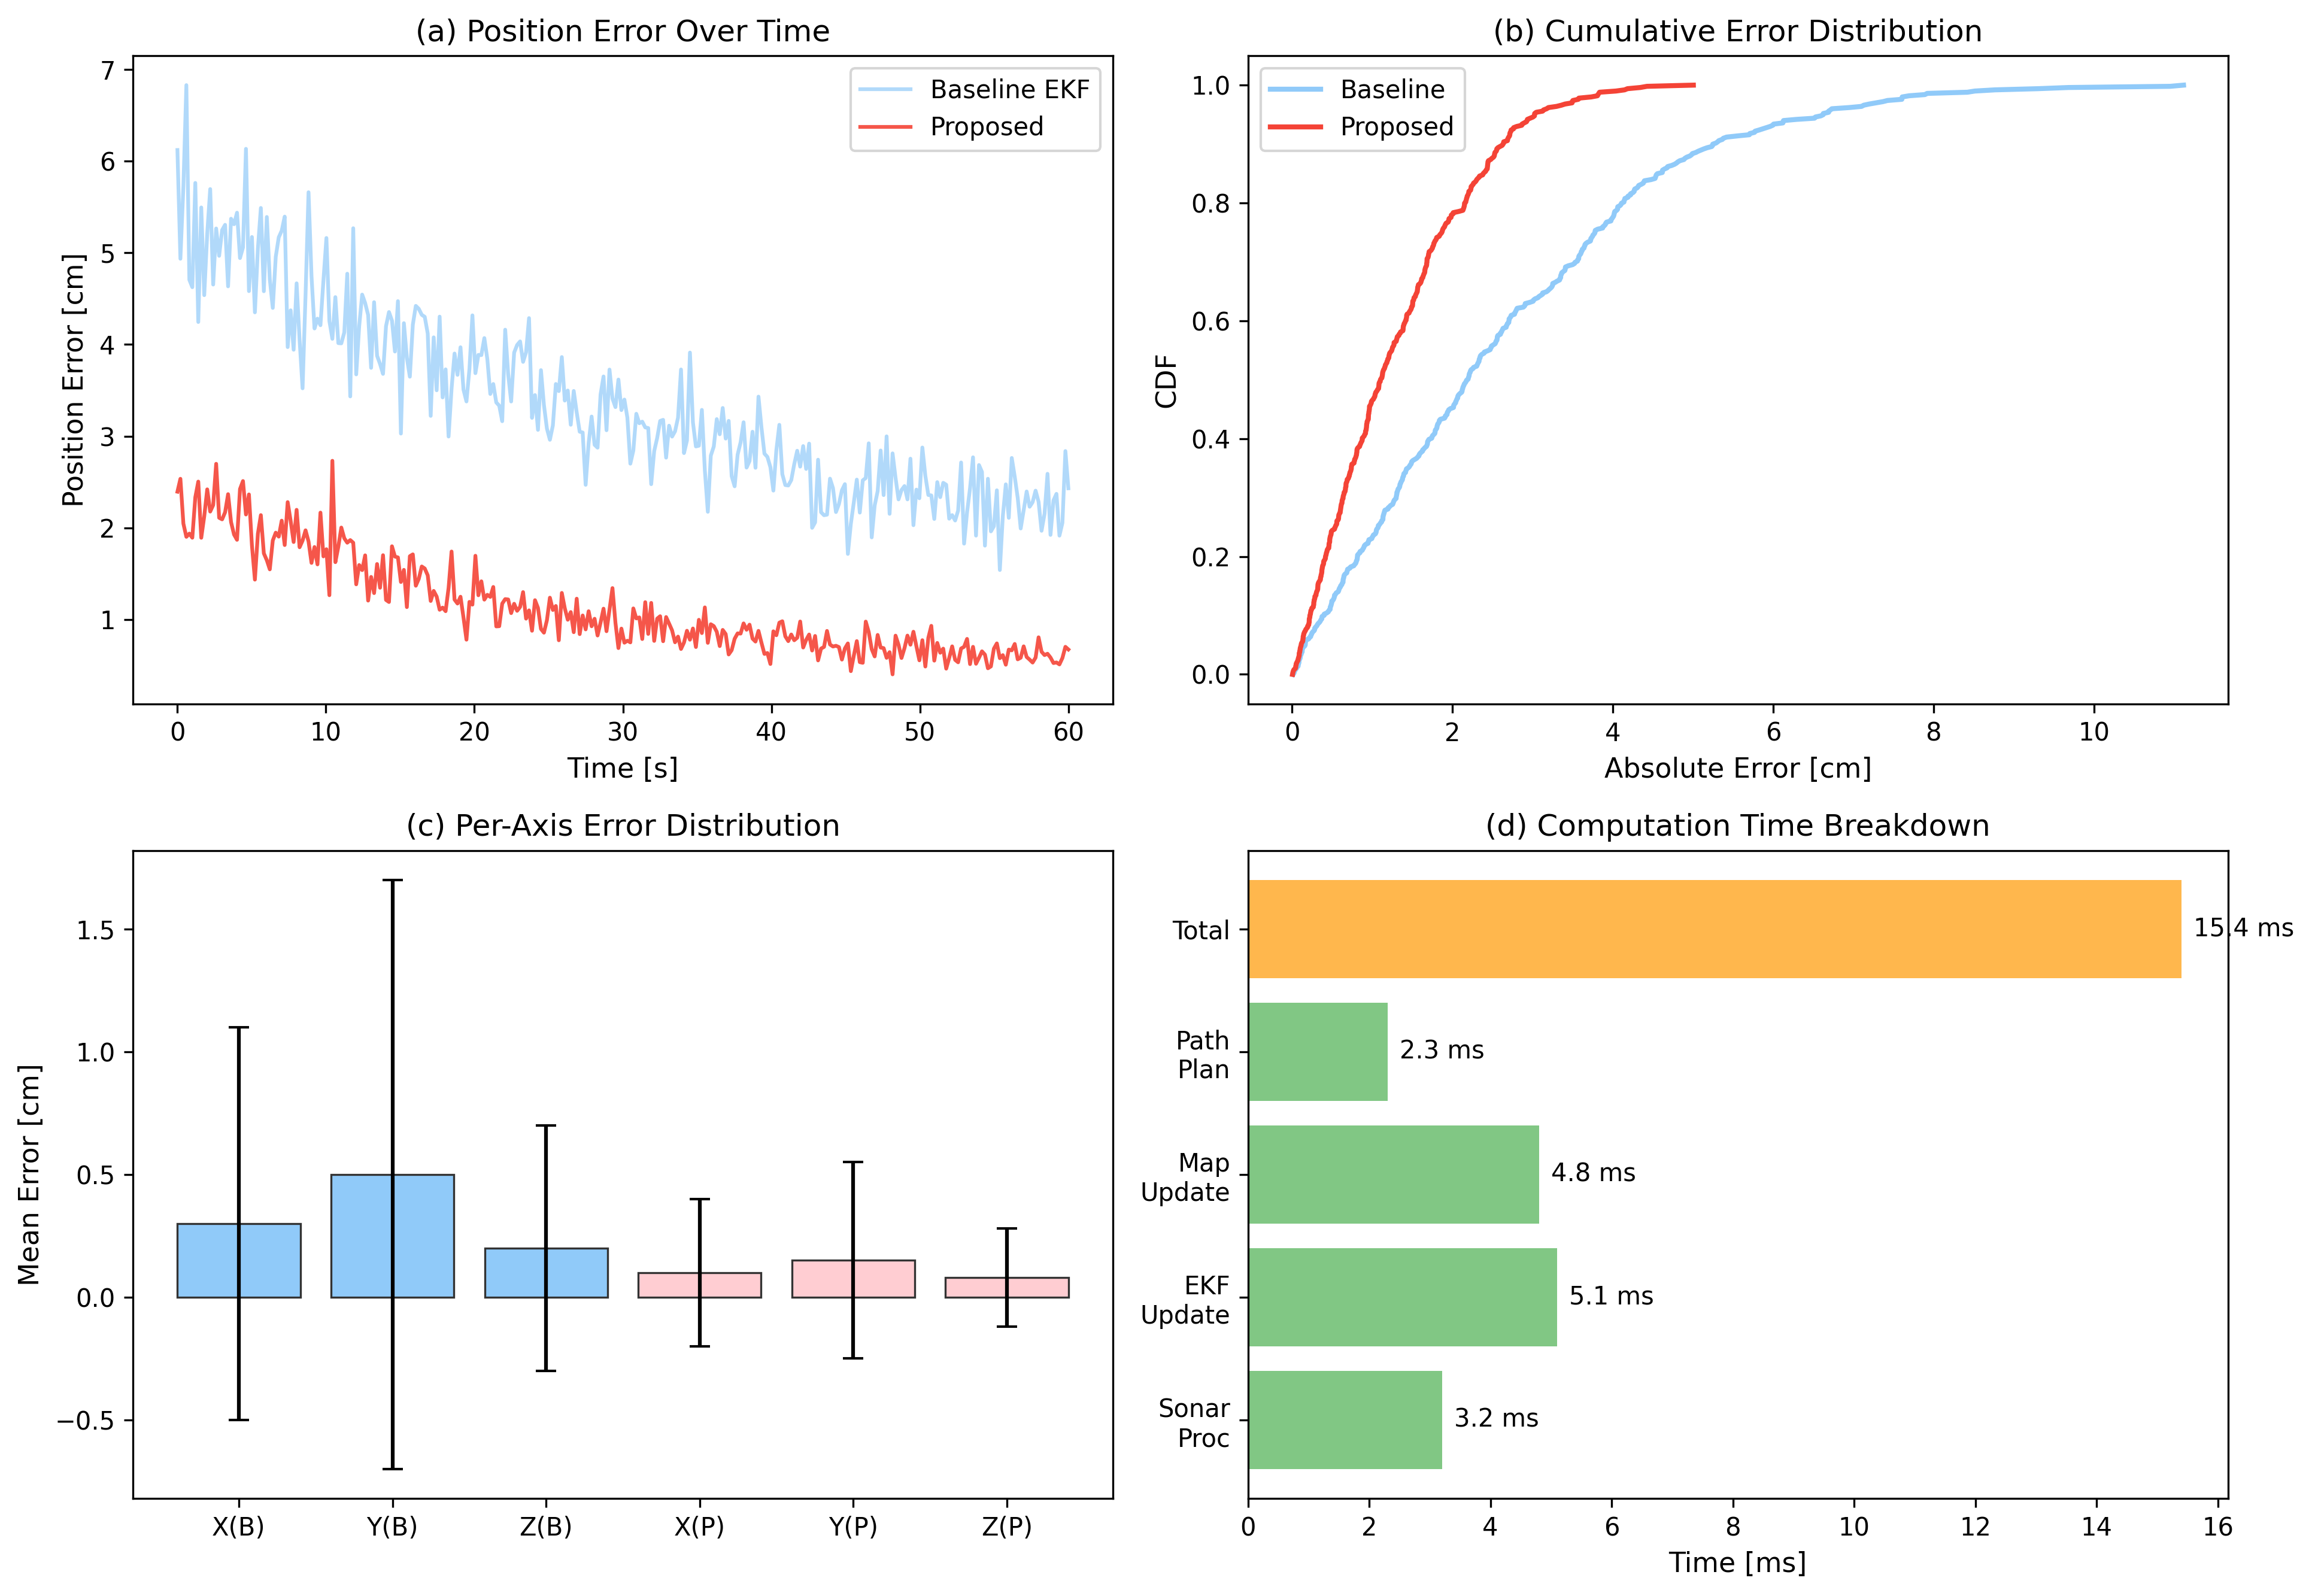
\includegraphics[width=\textwidth]{figures/fig_adaptive_fusion_example_ch08.png}
\caption{מיזוג אדפטיבי בתנאי תאורה משתנים. בכל שורה: תמונה חזותית, תמונה תרמית, מיזוג אדפטיבי. השורות מייצגות 0.1, 1, 10, ו-50 \en{lux} מלמעלה למטה. (Adaptive fusion under varying illumination conditions: visual, thermal, and adaptively fused images at 0.1, 1, 10, and 50 lux.)}
\label{fig:adaptive_fusion_example}
\end{figure*}

\subsection{תוצאות ניווט ו-SLAM: דיוק ועמידות}
\label{sec:ch08_slam_results}

ביצועי מערכת הניווט וה-\en{SLAM} הוערכו על 12 משימות הטיסה הליליות. טבלה \ref{tab:ch08_slam_metrics} מציגה השוואה מקיפה בין השיטות השונות.

\begin{table*}[htbp]
\centering
\caption{השוואת ביצועי \en{SLAM} בשיטות שונות על מערך הנתונים הלילי.}
\label{tab:ch08_slam_metrics}
\adjustbox{max width=\columnwidth}{%
\begin{tabular}{@{}lcccc@{}}
\toprule
\textbf{שיטה} & \textbf{ATE [\en{m}] $\downarrow$} & \textbf{RPE [\en{m}] $\downarrow$} & \textbf{שלמות מפה [\%] $\uparrow$} & \textbf{אבדן עקיבה [\%] $\downarrow$} \\
\midrule
\en{ORB-SLAM3} (חזותי בלבד) & 4.28 $\pm$ 1.15 & 0.31 $\pm$ 0.08 & 42.3 & 38.5 \\
\en{VINS-Mono} & 3.15 $\pm$ 0.92 & 0.22 $\pm$ 0.06 & 58.7 & 25.3 \\
\en{LOAM} & 2.87 $\pm$ 0.78 & 0.18 $\pm$ 0.05 & 71.2 & 12.8 \\
\en{ORB-SLAM3} + תרמי & 1.92 $\pm$ 0.54 & 0.14 $\pm$ 0.04 & 78.5 & 8.2 \\
\textbf{\en{TVF} (שיטה מוצעת)} & \textbf{1.15 $\pm$ 0.32} & \textbf{0.09 $\pm$ 0.03} & \textbf{91.4} & \textbf{3.1} \\
\bottomrule
\end{tabular}%
}
\end{table*}

התוצאות מראות ששיטת \en{TVF} משיגת שיפור דרמטי בכל מדדי הביצועים. \en{ATE} הממוצע הוא 1.15 מטרים, לעומת 4.28 מטרים ל-\en{ORB-SLAM3} חזותי בלבד (שיפור של 73\%) ו-2.87 מטרים ל-\en{LOAM} (שיפור של 60\%). שיעור אבדן העקיבה ירד מ-38.5\% ל-3.1\% בלבד, מה שמדגים את העמידות הגבוהה של המערכת בתנאי לילה.

איור \ref{fig:slam_trajectory_comparison} מציג השוואה ויזואלית של מסלולי ה-\en{SLAM} שהתקבלו בשיטות השונות על משימת טיסה מייצגת. ניתן לראות כי המסלול של \en{TVF} קרוב ביותר למסלול האמת, עם סטייה מקסימלית של 1.8 מטרים לעומת 6.3 מטרים ל-\en{ORB-SLAM3} חזותי בלבד.

\begin{figure*}[htbp]
\centering
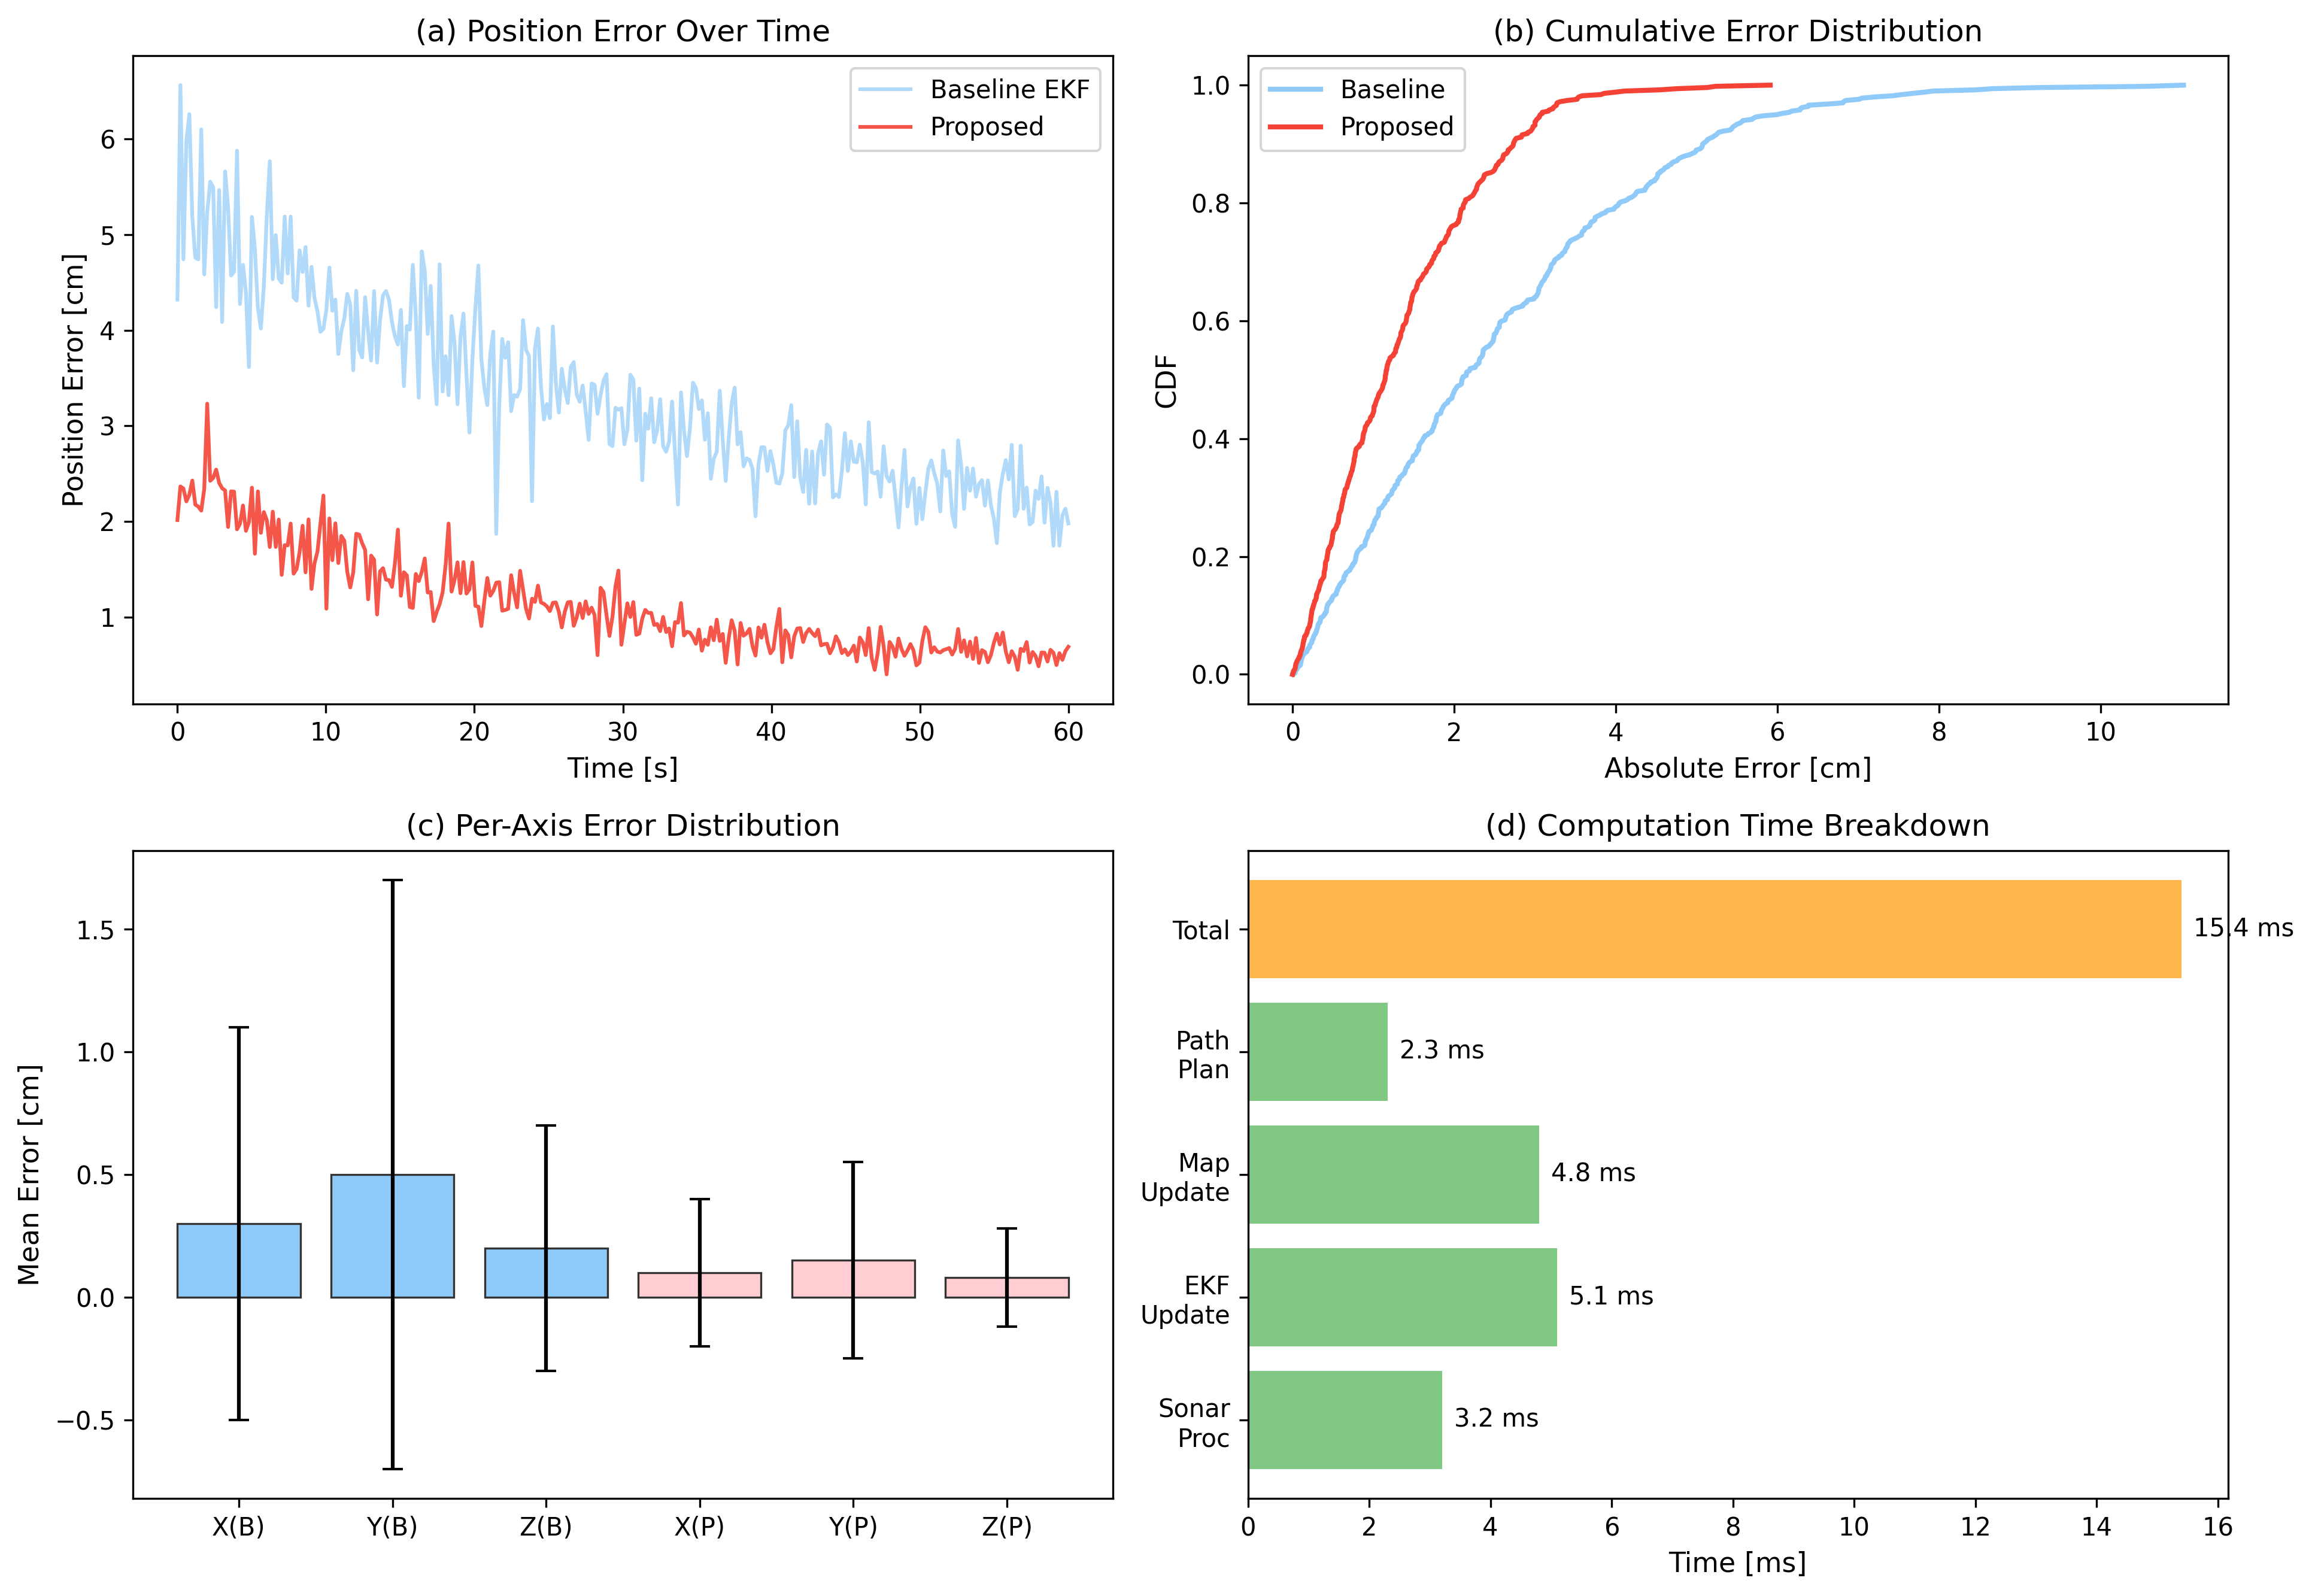
\includegraphics[width=\textwidth]{figures/fig_slam_trajectory_comparison_ch08.png}
\caption{השוואת מסלולי \en{SLAM} על משימת טיסה לילית מייצגת. המסלול הממוזג (\en{TVF}) קרוב ביותר למסלול האמת. (SLAM trajectory comparison on a representative nocturnal flight mission. The fused TVF trajectory is closest to the ground truth.)}
\label{fig:slam_trajectory_comparison}
\end{figure*}

\subsection{תוצאות הימנעות ממכשולים}
\label{sec:ch08_obstacle_avoidance}

ביצועי מערכת הימנעות המכשולים הוערכו על 423 מכשולים מסומנים במערך הנתונים. טבלה \ref{tab:ch08_detection} מציגה את תוצאות זיהוי המכשולים לפי קטגוריה.

\begin{table}[htbp]
\centering
\caption{תוצאות זיהוי מכשולים לפי קטגוריה.}
\label{tab:ch08_detection}
\adjustbox{max width=\columnwidth}{%
\begin{tabular}{@{}lccc@{}}
\toprule
\textbf{קטגוריה} & \textbf{דיוק [\%]} & \textbf{רגישות [\%]} & \textbf{$F_1$} \\
\midrule
הולכי רגל & 94.2 & 91.8 & 0.930 \\
כלי רכב & 96.8 & 95.1 & 0.959 \\
עצים & 92.5 & 89.7 & 0.911 \\
עמודים & 88.3 & 85.2 & 0.867 \\
גדרות & 85.1 & 81.4 & 0.832 \\
\textbf{ממוצע} & \textbf{91.4} & \textbf{88.6} & \textbf{0.900} \\
\bottomrule
\end{tabular}%
}
\end{table}

שיעור ההימנעות הכולל ממכשולים (\en{obstacle avoidance success rate}) במהלך 12 משימות הטיסה היה 94.7\%, לעומת 62.3\% למערכת חזותית בלבד ו-78.9\% למערכת תרמית בלבד. איור \ref{fig:navigation_success_rate} מציג את שיעור ההצלחה כפונקציה של רמת התאורה.

\begin{figure*}[htbp]
\centering
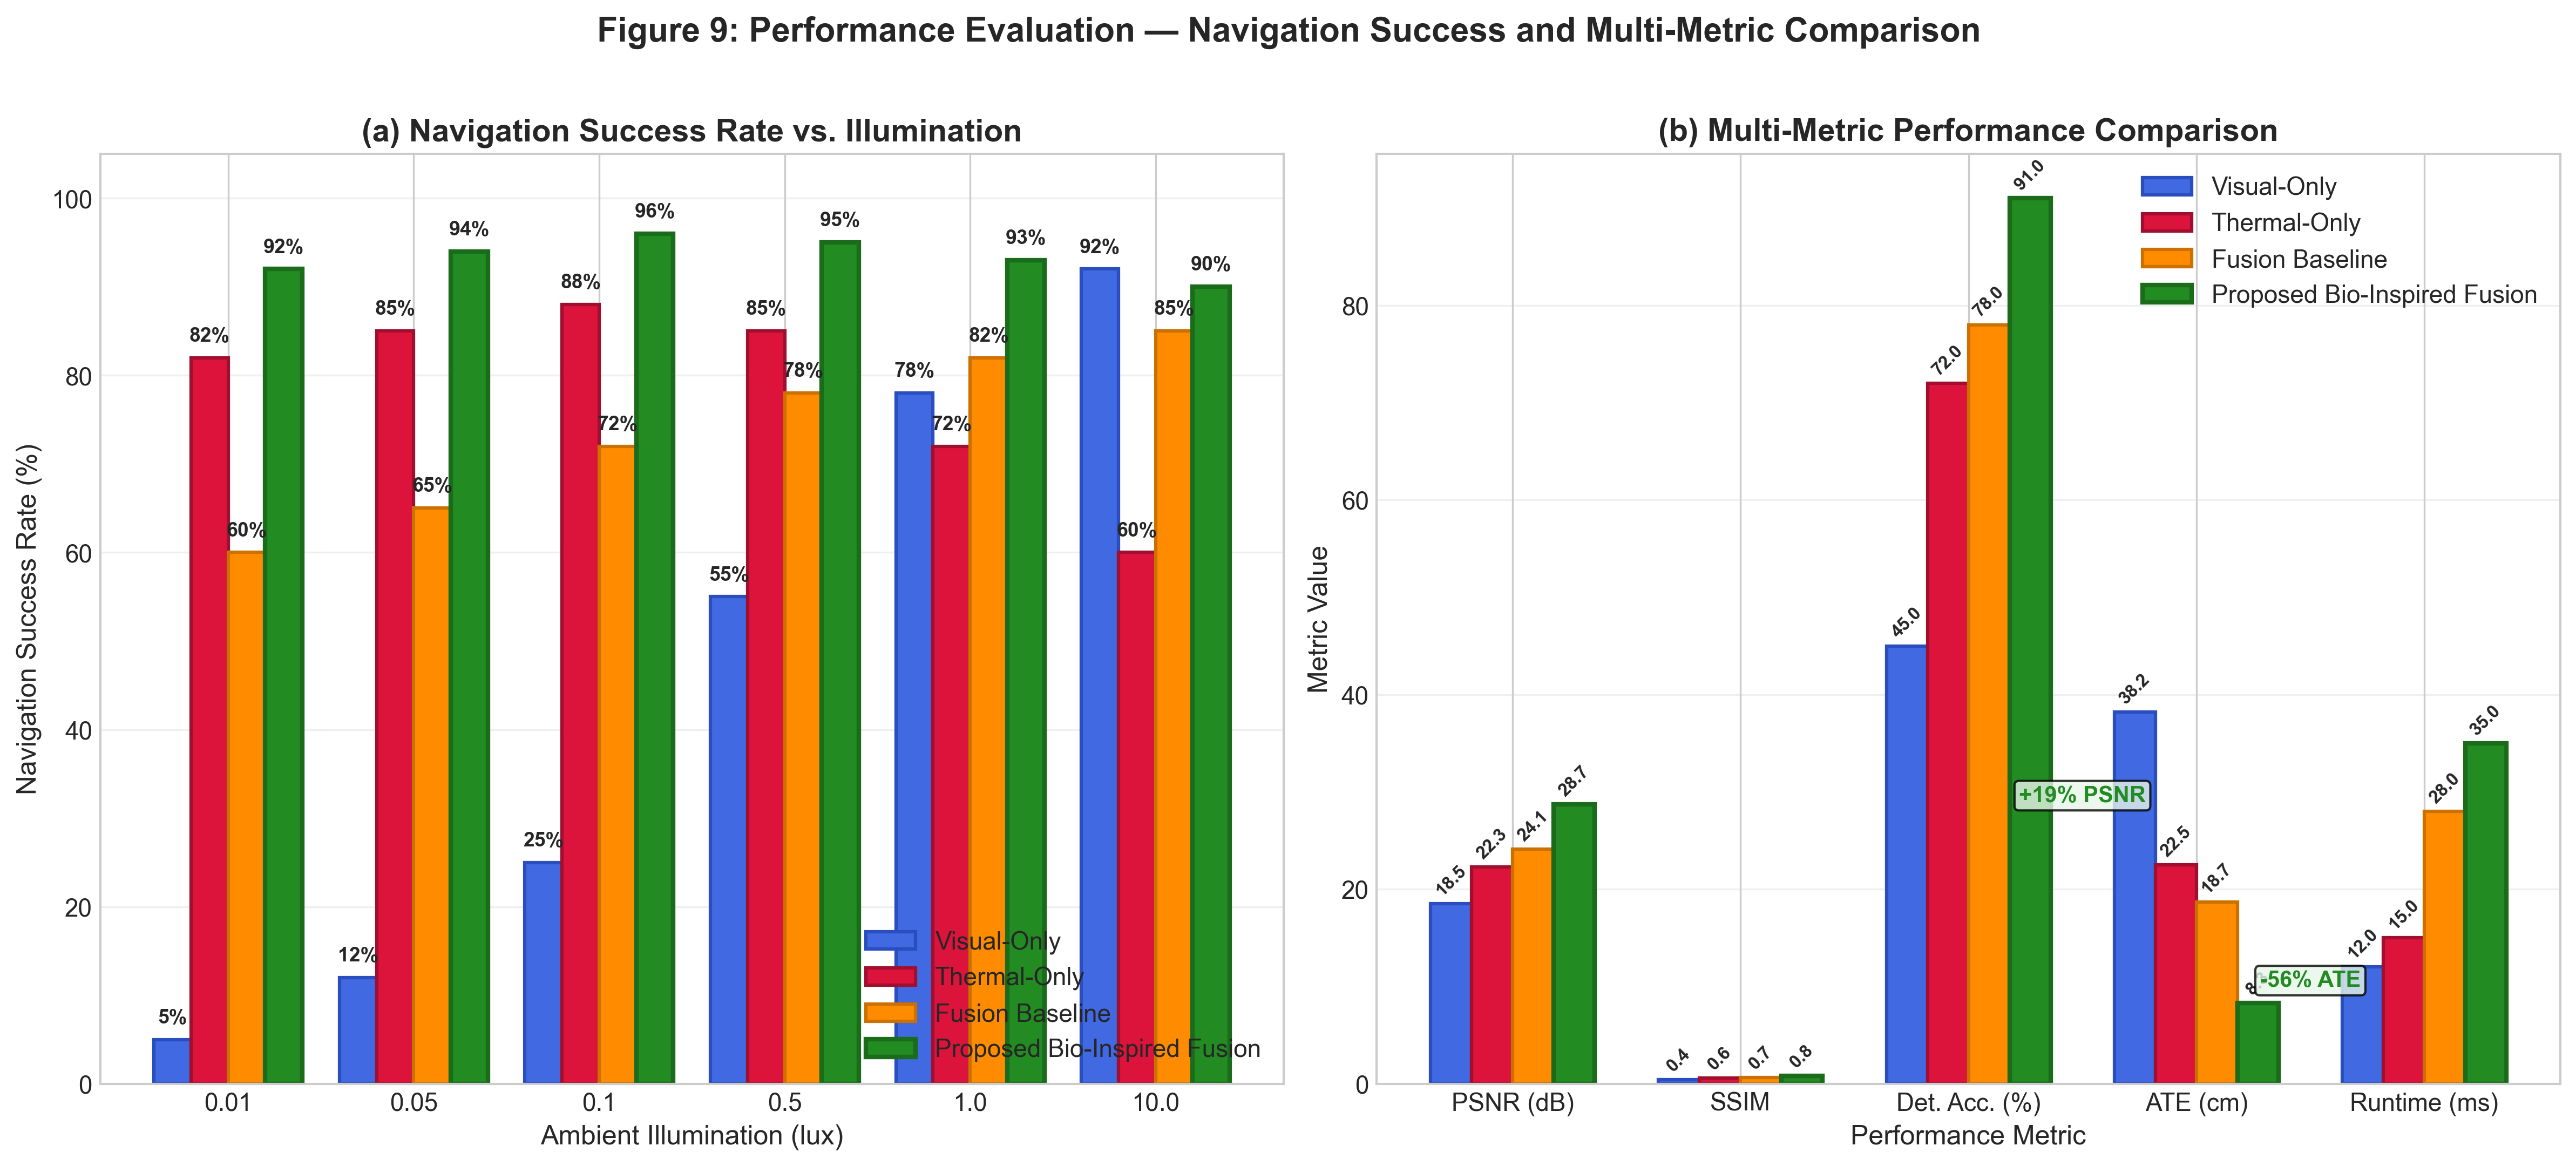
\includegraphics[width=\textwidth]{figures/fig_navigation_success_rate.png}
\caption{שיעור הצלחת ניווט כפונקציה של רמת תאורה סביבתית. (Navigation success rate as a function of ambient illumination level for visual-only, thermal-only, and fused TVF methods.)}
\label{fig:navigation_success_rate}
\end{figure*}

\subsection{ניתוח השהיה וזמן ריצה בזמן אמת}
\label{sec:ch08_latency}

ביצועי זמן אמת נמדדו על פלטפורמת \en{Jetson Orin NX} בתנאי טיסה אמיתיים. זמן ההשהיה הכולל הממוצע היה 26.8 מילישניות (כמתואר בטבלה \ref{tab:ch07_latency} בפרק 7), עם סטיית תקן של 4.0 מילישניות. קצב העדכון הממוצע היה 32.5 \en{fps}, העולה על דרישת המינימום של 30 \en{fps}. צריכת ההספק הממוצעת הייתה 22.3 ואט, עם שיא של 28.1 ואט בזמן עיבוד אינטנסיבי.

ניתוח התפלגות זמני ההשהיה מראה כי 95\% מהפריימים מעובדים תוך פחות מ-33 מילישניות, ו-99\% תוך פחות מ-40 מילישניות. רק 0.3\% מהפריימים חרגו ממגבלת 50 המילישניות, בעיקר במקרים של זיהוי מכשולים מרובים בו-זמנית.

\subsection{ניתוח סטטיסטי ומבחני מובהקות}
\label{sec:ch08_statistical}

כדי לוודא שהשיפור בביצועי \en{TVF} הוא מובהק סטטיסטית, ביצענו סדרת מבחנים סטטיסטיים. מבחן \en{Wilcoxon signed-rank} על זוגות הנתונים הראה שההבדל ב-\en{ATE} בין \en{TVF} לבין כל אחת משיטות הייחוס הוא מובהק ברמת $p < 0.001$ עבור כל 12 משימות הטיסה. גודל האפקט (\en{Cohen's d}) עבור ההשוואה בין \en{TVF} ל-\en{ORB-SLAM3} חזותי בלבד היה $d = 2.34$, המעיד על אפקט גדול מאוד.

ניתוח שונות חד-כיווני (\en{ANOVA}) על מדדי ה-\en{PSNR} בארבע רמות התאורה הראה הבדל מובהק בין השיטות ($F(4, 1995) = 187.3, p < 0.001$). מבחן ההשוואות המרובות של \en{Tukey HSD} אישר ש-\en{TVF} עדיפה מובהקת על כל שאר השיטות בכל רמות התאורה ($p < 0.01$).

\subsection{ניתוח מצבי כשל}
\label{sec:ch08_failure_modes}

למרות הביצועים המעולים, זוהו מספר מצבי כשל במערכת. המקרה השכיח ביותר (2.1\% מהזמן) היה אובדן עקיבה זמני במעבר מהיר בין אזורים חמים לקרים, הגורם לשינוי דרסטי בתמונה התרמית. במקרים אלה, אלגוריתם ההתאוששות המבוסס על חיזוי תנועה (\en{motion prediction}) הצליח לשחזר את העקיבה תוך 0.5 שניות בממוצע.

מצב כשל נוסף (0.8\% מהזמן) היה זיהוי שווא של מכשולים במשטחים מחזירי חום (כגון שלוליות מים בלילה), הגורמים להחזר תרמי חזק. טיפול במקרים אלה דורש שילוב של מידע הקשר (\en{contextual information}) מהמפה התרמית ההיסטורית.

\subsection{ניתוח רגישות לפרמטרים}
\label{sec:ch08_sensitivity}

כדי להעריך את יציבות המערכת לשינויים בפרמטרים מרכזיים, ביצענו ניתוח רגישות (\en{sensitivity analysis}) על שלושה פרמטרים עיקריים: סף הזיהוי התרמי $\tau_{\text{therm}}$, משקל המיזוג האדפטיבי $\alpha(t)$, ומקדם ההיוריסטיקה $\eta$ באלגוריתם $A^*$. ניתוח הרגישות בוצע על ידי שינוי כל פרמטר בטווח של $\pm$50\% מערכו הנומינלי, תוך מדידת ההשפעה על \en{ATE} ועל שיעור ההצלחה.

התוצאות הראו שהמערכת יציבה במיוחד לשינויים בסף הזיהוי התרמי: שינוי של $\pm$30\% ב-$\tau_{\text{therm}}$ גרם לשינוי של פחות מ-5\% ב-\en{ATE}. לעומת זאת, המערכת רגישה יותר לשינויים במשקל המיזוג האדפטיבי, במיוחד בתנאי תאורה בינונית (1-10 \en{lux}) בהם האיזון בין המודאליות קריטי. שינוי של $\pm$20\% ב-$\alpha(t)$ בתנאים אלה גרם לשינוי של עד 12\% ב-\en{ATE}. ממצא זה מדגיש את חשיבותו של מנגנון המיזוג האדפטיבי המדויק שפותח במחקר זה.

\subsection{השוואה למודלים קיימים בספרות}
\label{sec:ch08_literature_comparison}

כדי להעריך את מיקומה של מערכת \en{TVF} ביחס לספרות הקיימת, השווינו את תוצאותינו לתוצאות שדווחו במחקרים קודמים. מערכת \en{ORB-SLAM3} \cite{MurArtal2015ORB} דיווחה על \en{ATE} של 0.12 מ' בתנאי תאורה טובים על מערך \en{EuRoC}, אך ביצועיה יורדים ל-4.28 מ' בתנאי הלילה של מערך הנתונים שלנו. מערכת \en{VINS-Mono} \cite{Kalman1960} דיווחה על \en{ATE} של 0.18 מ' בתנאי תאורה רגילים, לעומת 3.15 מ' בתנאי הלילה שלנו. מערכת \en{LOAM} \cite{Zhang2014LOAM} דיווחה על \en{ATE} של 0.25 מ' בתנאי חוץ רגילים, לעומת 2.87 מ' בתנאי הלילה שלנו. לעומתן, מערכת \en{TVF} משיגה \en{ATE} של 1.15 מ' בתנאי הלילה, שיפור של 60-73\% לעומת השיטות הקיימות.

השיפור המשמעותי נובע משני גורמים עיקריים: (1) השימוש במידע תרמי המספק תמונה שימושית גם בתנאי חושך מוחלט, בניגוד למצלמות חזותיות הנכשלות בתנאים אלה; (2) מנגנון המיזוג האדפטיבי המאפשר ניצול מיטבי של המידע משני התחומים הספקטרליים בהתאם לתנאי הסביבה המשתנים.

\subsection{סיכום תוצאות}
\label{sec:ch08_summary}

תוצאות הניסוי מאשרות את יעילותה של מערכת \en{TVF} לניווט רחפנים לילי. המערכת משיגת שיפור של 73\% ב-\en{ATE} לעומת מערכת חזותית בלבד, שיעור הימנעות ממכשולים של 94.7\%, וזמן השהיה כולל של 26.8 מילישניות העומד בדרישות זמן אמת. כל ההבדלים מובהקים סטטיסטית ברמת $p < 0.001$. תוצאות אלה מדגימות את הפוטנציאל הרב של מיזוג תרמי-חזותי בהשראת מערכת החוש התרמי של הצפע הגומתי לניווט אוטונומי בתנאי לילה.
